\chapter{Neural Network Solution}

We will now explore how to use deep neural networks to price our American put options. Using the Black-Scholes dynamics we can derive the variational equation, a partial differential equation that our solution must satisfy. As the solution of this PDE does not have a closed form in general, we aim to find an approximation to the solution by using a neural network. This can be done by customising a loss function as the variational equation, along with some boundary conditions that we know our value function must satisfy, with the hope that using optimisation techniques such as gradient descent, we can approach the solution numerically by descending the loss landscape.

\section{Variational Equation}

copied over already

\section{Black-Scholes Operator}

To obtain the variational equation for multiple assets, we can follow the same steps as we did for the one-dimensional case. Consider a derivative on $k$ underlying assets whose price vector $S = (S^1 , \dots, S^k)^\top$ follows a geometric Itô diffusion under the risk-neutral measure $\mathbb Q$. Formally, the asset prices solve the SDEs under $\mathbb Q$:

\[
\mathrm dS_t^i = rS_t^i\mathrm dt + \sigma_i S^i_t \mathrm dW_t^i
\]

where we can introduce correlation into the assets by

\[
\mathbb E\big[\mathrm dW_t^i \mathrm dW_t^j\big] = \rho_{ij}\mathrm dt
\]

As before, denote $g:\mathbb R^k_+ \to \mathbb R$ the payoff on exercise and $T>0$ the time of maturity. The value function stays

\[
v(t, S) = \sup_{\tau \in [t, T]} \mathbb E_t\big[e^{-r(\tau - t)}g(S_\tau)\big]
\]

By following the 1D case, should we choose not to exercise the option and proceed to $t+h$ for a small $h > 0$, we can apply Ito’s lemma on multiple dimensions to yield

\[
v(t+h, S_{t+h})= v(t, S) + \int_t^{t+h} \left(\frac{\partial v}{\partial t}(u, S_u) + \mathcal L_u v(S_u)\right)\,\mathrm du
\]

where, for convenience, we have the Black-Scholes ordinary differential operator $\mathcal L$ acting on $S$ with

\[
\mathcal L_uv(S_u) = \sum_{i=1}^k\frac{\partial v}{\partial S^i}(u, S_u)rS_u + \frac 12 \sum_{i=1}^k\sum_{j=1}^k \frac{\partial^2 v}{\partial S^i\partial S^j}(u, S_u) \sigma_i\sigma_j \rho_{ij} S^i_uS^j_u
\]

and the linear parabolic operator $\mathcal G$ has the analogous definition as to the 1D case:

\[\mathcal G[v]:= rv(t, S) - \frac{\partial v}{\partial t}(t, S) - \mathcal L_tv(S)\]

We can thus, using the same steps as the 1D case, yield the variational equation for multiple dimensions to be the same thing:

\[
\min\left(\mathcal G[v], v(t, S)  - g(S)\right) = 0
\]

with the terminal condition $v(T, S) = g(S)$.


\section{Implementation}

To use a neural network to approximate the function $v(t, S)$, we need to establish a loss function that would help our estimate converge to the solution. As mentioned before, this loss function should take both the variational equation and the boundary conditions into account. The boundary conditions would of course depend on the payoff of the derivative specifically, but for an American put option it has the general structure:

\begin{itemize}
    \item Variational loss ($J_1$): the value we obtain when we plug the current function represented by the neural network into the variational equation.
    \item Exercise loss ($J_2$): the value at the expiry should just be the payoff.
    \item Max boundary loss ($J_3$): the value of the derivative at the upper bound of the stock price should be $0$ at any time, as we assume the option will expire out of the money.
    \item Min boundary loss ($J_4$): the value of the derivative at the lower bound of the stock price should be the payoff at any time, as early exercise is always good here.
\end{itemize}

Taking this into account, we will train our network over a set number of iterations where in each iteration, we will implement stochastic gradient descent by sampling a batch of $B$ points for both the time and the stock prices, which would be used to approximate the loss that we descend, which is the weighted sum of the four components
\[J = \sum_{i=1}^4 \lambda_iJ_i\]
for $\bm \lambda = (\lambda_1, \dots, \lambda_4) \in \Delta^4$, the unit simplex. These weights are to be tuned so that no component of the loss function is dominating the loss and we get a better fit.

\subsection{One dimension}

We will approximate the four loss components by sampling $B$ points each epoch and computing the mean squared error of the loss contributions. For this, we will choose our batch size to be $B=1000$ to obtain our sample points for epoch $i$
\begin{align*}
    (t_1^{(i)}, \dots, t_B^{(i)}) &\in [0, T]^B\\
    (S_1^{(i)}, \dots, S_B^{(i)}) &\in [S_\text{min}, S_\text{max}]^B
\end{align*}

where $S_\text{min}, S_\text{max} \in [0, \infty)$ are parameters which we assume to be the minimum and maximum possible values of the stock respectively between now and expiry. To obtain these samples, we can consider various sampling schemes [add details]:

\begin{itemize}
    \item Uniform distribution
    \item Truncated normal
\end{itemize}

With our batch of samples $(t_1^{(i)}, \dots, t_B^{(i)})$ and $(S_1^{(i)}, \dots, S_B^{(i)})$, the loss components in epoch $i$ can be computed as the MSE:

\begin{align*}
J_1^{(i)} &= \frac 1B\sum_{j=1}^B\left\|
\min\left(\mathcal G[f], f(t_j^{(i)}, S_j^{(i)}) - g(S_j^{(i)})\right)
\right\|^2_2 \\
J_2^{(i)} &= \frac 1B\sum_{j=1}^B \| f(T, S_j^{(i)}) - (K-S_j^{(i)})^+\|^2_2\\
J_3^{(i)} &= \frac 1B\sum_{j=1}^B \|f(t_j^{(i)}, S_\text{max}) \|^2_2\\
J_4^{(i)} &= \frac 1B\sum_{j=1}^B \| f(t_j^{(i)}, S_\text{min}) - (K-S_\text{min})\|^2_2\\
\end{align*}

with $J^{(i)} = \sum_{i=1}^4 \lambda_i^{(i)} J_i^{(i)}$ as before, where our weights $\bm \lambda^{(i)} \in \Delta_4$ can either be constant or evolve dynamically. For simplicity, we choose them to be constant after tuning. We will use the ReLU activation function, the Adam optimiser with default parameters and learning rate $0.001$.

\subsection{Loss in multiple dimensions}

Again, we will sample $B$ points per epoch to approximate the loss components for each epoch. A batch size of $B=1000$ works similarly well for our purposes. We will introduce the notation for our samples on $k$ assets:
\begin{align*}
    (t_1, \dots, t_B) &\in [0, T]^B\\
    (\bm S_1, \dots, \bm S_B) &\in [S^1_\text{min}, S^1_\text{max}]\times \cdots \times [S^k_\text{min}, S^k_\text{max}]
\end{align*}

where $\bm S_j = (S_j^1, \dots, S_j^k)$. We would like to price the price of the put on the product of these $k$ assets, so let's additionally introduce the product
\[X_j = \prod_{i=1}^k S_j^i\]
where we can additionally have $X_\text{min} = \prod_{i=1}^k S_\text{min}^i$ and $X_\text{max} = \prod_{i=1}^k S_\text{max}^i$.
For simplicity, all of these samples will be generated iid and uniformly in their respected domains. Given these samples, the loss components can be extended to $k$ dimensions:

\begin{align*}
    J_1 &= \frac{1}{B} \sum_{j=1}^B \left\| \min \left(\mathcal G[f], f(t_j, \bm S_j) - g(\bm S_j\right)\right\|_2^2 \\
    J_2 &= \frac 1B \sum_{j=1}^B \left\| f(T, \bm S_j) - (K - X_j)^+\right\|_2^2 \\
    J_3 &= \frac 1B \sum_{j=1}^B \left\| 
    f(t_j, \bm S_j) \mathbb I_{\{X_j > 0.8X_\text{max}\}} \right\|_2^2 \\
    J_4 &= \frac 1B \sum_{j=1}^B \left\|\left( f(t_j, \bm S_j) - (K - X_j)^+\right)\mathbb I_{\{\exists i : S^i_j = S^i_\text{min}\}}\right\|_2^2
\end{align*}

where $\mathbb I_{A}$ is the indicator function for the event $A$. The first two components, $J_1$ and $J_2$ are analogous to the 1D case. For the third component, we will only penalise if the product of the assets is close to some threshold, which we choose to be $0.8$ of the maximum possible product of asset prices. The fourth component enforces immediate exercise as long as one of the assets is at its minimum theoretical price, which would be done by selecting an asset uniformly randomly in each sample and setting that to the corresponding modelled minimum price.

Again, our total loss for the epoch is the weighted sum of these four components, and we will again use the ReLU activation function, the Adam optimiser with default parameters and learning rate $0.001$.

\section{Numerical Results}

\clearpage

\section{Free Boundary}

We are now interested in finding the free boundary of the American put option, which is the boundary separating the exercise region and the continuation region. For an initial visualisation, assume the risk-neutral dynamics of our asset $S$ is modelled as a geometric brownian motion with constant risk-free interest rate $r$ and volatility $\sigma$. As before, the value of the American put with strike $K$ and maturity $T$ is given by the optimal stopping problem

\[v(0, S) = \sup_{\tau \in [0, T]} \mathbb E\big[e^{-r\tau}(K - S_\tau)^+\big] \]

which is achieved by an optimal stopping time $\tau^\star$ taking the form

\[\tau^\star = \inf\{t \ge 0 : S(t) \le b^\star(t)\}\]

for some optimal exercise boundary $b^\star(t)$ \cite{glasserman2004monte}. This is illustrated in Figure \ref{fig:free_boundary}, where we simulate one realisation of the asset price and plot it against the exercise boundary, which is found using binary search on the binomial tree solution, where we have

\[b^\star(t) = \inf\{S : v(t, S) > g(S)\}\]

because as soon as the option has no time value, it is optimal to exercise.

\begin{figure}[h!]
    \centering
    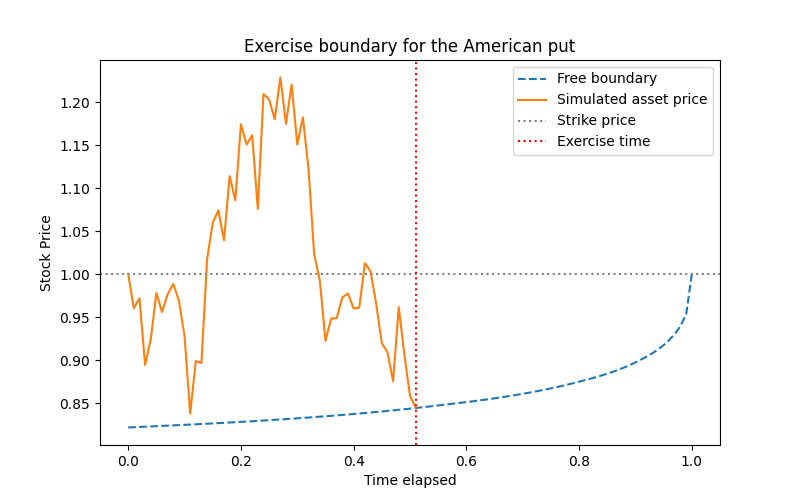
\includegraphics[width=0.8\textwidth]{../plots/free_boundary.png}
    \caption{Exercise boundary for the American put}
    \label{fig:free_boundary}
\end{figure}

This formulation describes a hard classification problem, where we classify points in the time-stock price space binarily to be either in the continuation region or the exercise region. However, our numerical solutions to the pricing problem are not exact and there is some level of error in the solution that comes from the Monte Carlo simulations upon the space, the numerical differentiation used in training and the early stopping in the training process. Therefore, it would be more intuitive to perform a soft classification instead, where we assign probabilities to points in the time-stock price space to be in the continuation region or the exercise region, which would give us a more intuitive visualisation of the free boundary and how it evolves over time. We will do this by extending hard classification: that is to say, the continuation region $A$ is

\[A = \{(t, S) : u(t, S) > g(S)\} \cup \{(t, S) : g(S) = 0\}\]

where intuitively the first term indicates that we still have time value, and the second term immediately assigns at-the-money and out-of-the-money options in the continuation region as they are worthless under immediate exercise.

To extend the definition of the continuation region to a soft classification, we consider the sigmoid function $s: \mathbb R \to (0, 1)$ defined as

\[ s(x) = \frac{1}{1 + e^{-x}}\]

and introducing two softness parameters $\tau_1, \tau_2 > 0$ to yield our continuation probability function on the relative difference from the payoff as

\[ P_\text{cont}(d) = \begin{cases}
    s \left(\frac{d}{\tau_1}\right) & d \le 0 \\
    s \left(\frac{d}{\tau_2}\right) & d > 0
\end{cases}, \qquad d := \frac{u(t, S) - g(S)}{g(S)}\]

We introduce different softness paramaters depending on the sign of $d$ because we would like different leniencies for when the value function is above or below the payoff. Value functions below the payoff arise under errors in the neural network solution and thus our continuation probability should be steeper.

These softness parameters can be determined by defining thresholds $\epsilon_1, \epsilon_2 > 0$ such that for $I \in (0.5, 1)$ we have

\[P_\text{cont}(-\epsilon_1) = 1-I, \qquad P_\text{cont}(\epsilon_2) = I\]

which we could solve with some simple algebraic manipulation to get

\[ \tau_1 = \frac{\epsilon_1}{\ln\left(\frac{I}{1 - I}\right)}, \qquad \tau_2 = \frac{\epsilon_2}{\ln\left(\frac{I}{1 - I}\right)}\]

These classifications are illustrated in Figure \ref{fig:continuation_probabilities}, where we can see that the continuation probabilities are close to $1$ in the continuation region and close to $0$ in the exercise region, with a smooth transition between the two regions. We can see that even though the neural network solution correctly captures the regional behaviour of the value function, it struggles with estimating the time value of the option, which can be observed by the fact that the free boundary curve is concave rather than convex.

\begin{figure}[h!]
    \centering
    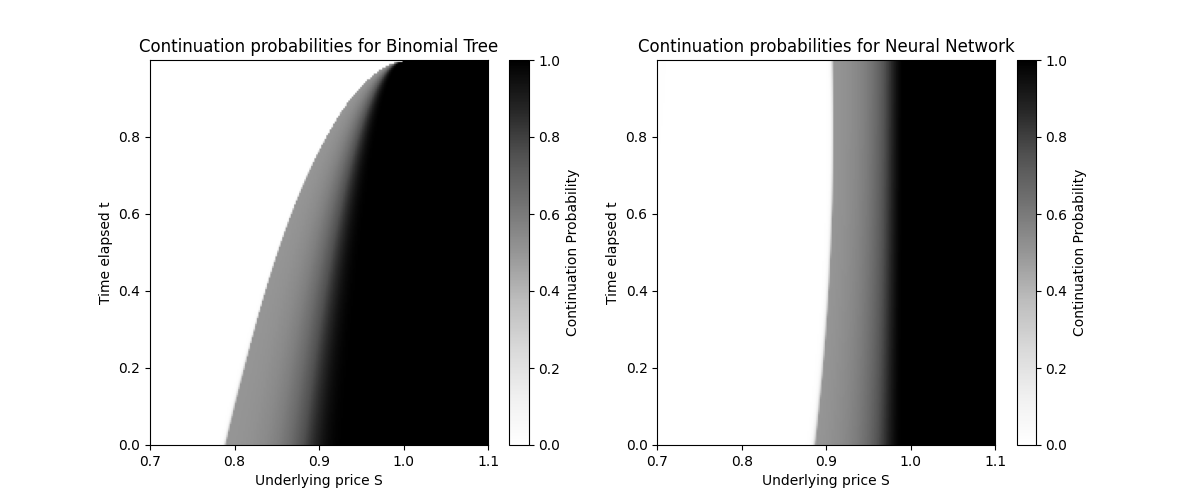
\includegraphics[width=\textwidth]{../plots/continuation_probabilities.png}
    \caption{Continuation probabilities for the American put}
    \label{fig:continuation_probabilities}
\end{figure}